\chapter{实验测试与分析}
\label{sec:Experiment}

在本章中,将给出基于真实世界数据集的评估结果,以证明本文针对加密重复数据删除提出的频率分析攻击方法的有效性(对加密重复数据删除的威胁的严重性)。

\section{实验方法}
\label{sec:dataset}

本文所使用的真实世界数据集不包数据的实际内容,因此基于数据块哈希模拟攻击者所拥有的的对抗性知识。具体来说,本文将一些快照中的有序的数据块哈希列表作为辅助信息$\mathbf{A}$和原始明文信息$\mathbf{M}$。为了模拟加密过程,在$\mathbf{M}$中的每个原始数据块哈希(表示明文)上应用额外的哈希函数,并将结果截断为当前使用的数据集中约定的哈希值的长度。截断的结果用于模仿$\mathbf{C}$中的密文。对于每个推断的密文数据块-明文数据块对$(C,M)$,本文通过在$M$上应用相同的模拟加密并将结果与​​$C$进行比较来验证其正确性。特别的,基于聚类的频率分析攻击可以在数据段级别进行操作,断出密文数据段-明文数据段对$(S_\mathbf{C},S_\mathbf {A})$。在这种情况下,本文通过检查$S_\mathbf{C}$中的每个密文是否完全映射到$S_\mathbf{A}$中的每个明文来评估$(S_\mathbf {C},S_\mathbf{A})$的正确性。

本文通过推理率和推理精度两个标准来衡量攻击的有效性(参见\ref{sec:ThreatModel})。


\section{基于分布的攻击的实验结果}
\label{sec:experiment-distribution}

\subsection{实验1(参数的影响)}


本节将评估参数$(u, r, t)$的变化在基于分布的频率分析攻击中带来的影响。实验使用FSL数据集(参见\ref{sec:fsl})来进行评估。在实验中使用每个用户的第12周备份作为辅助信息来推断该用户相应的第14周备份中的原始明文数据。出于控制变量的需求,实验将在固定另两个参数的前提下对三个参数中的一个的变化进行测试和分析。


\subsubsection{参数$u$的影响}

首先,配置参数$t \rightarrow \infty$和$r = 0$来评估参数$u$变化的影响(在这种情况下,基于分发的攻击将退化到基于数据块局部性的的攻击\cite{li2017information})。

\begin{figure}[!htbp]
    \centering
    \begin{tabular}{p{.48\linewidth}p{.48\linewidth}}
        \multicolumn{2}{c}{
\includegraphics[width=.7\textwidth]{legend-fsl-line.pdf}}  \\
        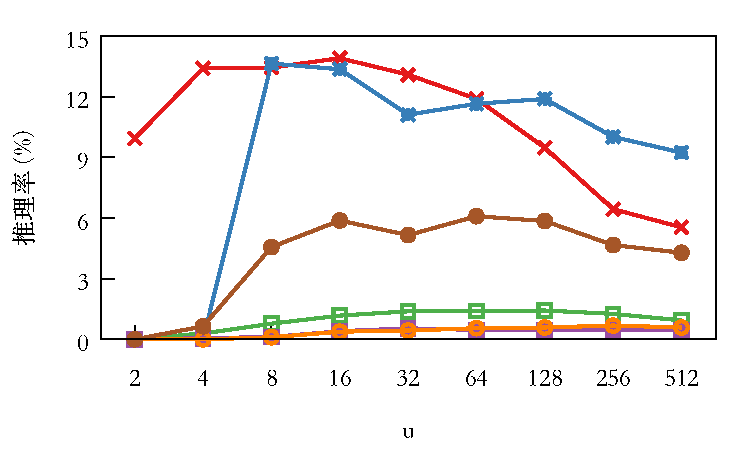
\includegraphics[width=\linewidth]{dis-impact-u-rate.pdf} &
        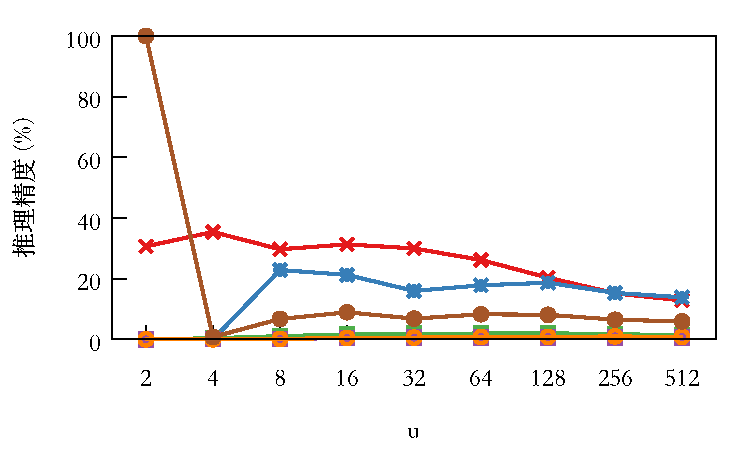
\includegraphics[width=\linewidth]{dis-impact-u-accuracy.pdf}\\
    \end{tabular}
    \caption{基于分布的攻击实验1-参数$u$的变化对推理结果的影响($r = 0$;$t \rightarrow \infty$)}
    \label{fig:distribution-impact-u}
\end{figure}

图\ref{fig:distribution-impact-u}显示了将参数$u$从2变为512时对推理率和推理精度带来的影响。对于推理率的结果,本实验的观察结果与已有的工作\cite{li2017information}相同。推理率首先随着$u$的增大而提高,这是因为频率分析攻击可以推断出更多的密文数据块-明文数据块对。推理率在达到最大值之后(例如,User004为13.9\%,User007为13.6\%,User012为1.4\%,User013为0.5\%,User015为0.7\%,User028为6.1\%)开始下降。其原因在于频率分析引入了大量的误报,这些误报会继续影响基于分布的攻击对每个数据块相邻邻居的推断。同时,部分特殊情况下的推理率约为0.0001\%,这意味着攻击只能推断出几个密文数据块-明文数据块对。

已有的工作\cite{li2017information}不提供基于数据块局部性的攻击的推理精度信息,因此本文提出的两种推理攻击方法的实验的推理精度的部分不与其进行对比。实验中观察到除User028的数据在$u=2$的条件下没有引入任何误报外,针对所有用户备份数据的推理精度都处于相当低的水平(小于40\%)。随着$u$的增大,推理精度会略有下降。例如,当$u$从2增加到512时,User004的推理精度从30.7\%下降到12.8\%。
    
{\bf Observation (1) --} 

A relatively larger $u$ increases the inference rate, yet it decreases the inference precision (i.e., more false positives are introduced). 


\subsubsection{参数$r$的影响}

Informed by the impact of $u$, we set $u$ at 128 for User004, User013 and User015, and at 256 for User007, User012 and User028, respectively, in order to evaluate the impact of $r$ and $t$.  Our rationale is to increase the coverage of inferred ciphertext-plaintext pairs, while we use $r$ and $t$ to filter possibly false positives. 

\begin{figure}[!htbp]
    \centering
    \begin{tabular}{p{.48\linewidth}p{.48\linewidth}}
        \multicolumn{2}{c}{
\includegraphics[width=.7\textwidth]{legend-fsl-line.pdf}}  \\
        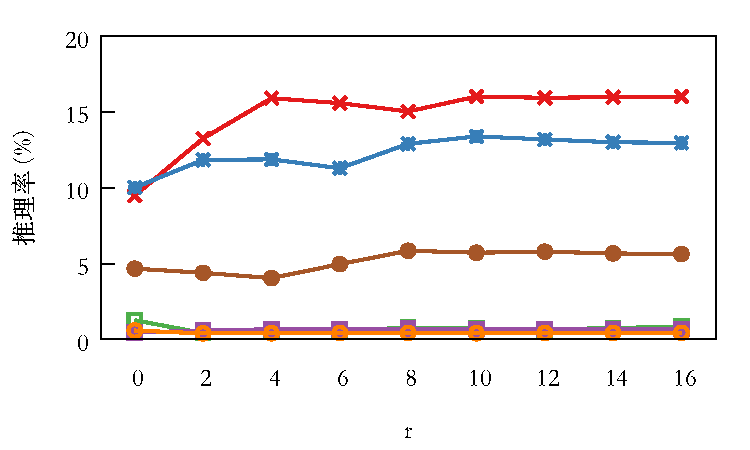
\includegraphics[width=\linewidth]{dis-impact-r-rate.pdf} &
        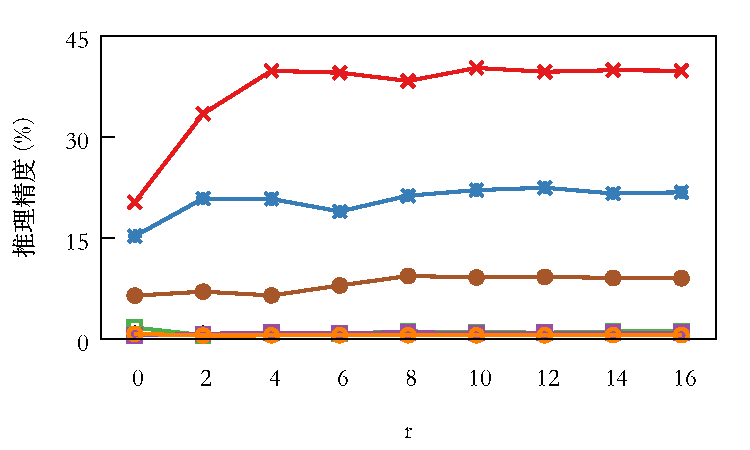
\includegraphics[width=\linewidth]{dis-impact-r-accuracy.pdf}\\
    \end{tabular}
    \caption{基于分布的攻击实验1-参数$r$的变化对推理结果的影响(User004、User013和User015中$u = 128$,User007、User012和User028中$u = 256$;$t \rightarrow \infty$)}
    \label{fig:distribution-impact-r}
\end{figure}

We first configure $t \rightarrow \infty$ and evaluate the impact of $r$. Figure~\ref{fig:distribution-impact}(b) shows the results. We observe that the inference rates of majority users increase with $r$. For example, when we vary $r$ from 0 to 16, the inference rates grow from 9.5\% to 16.0\%, from 10.0\% to 13.0\%, from 0.5\% to 0.7\%, and from 4.7\% to 5.6\% for User004, User007, User013, and User028, respectively. The reason is that the distribution-based attack addresses disturbances to frequency ranking, and infer more correct ciphertext-plaintext  pairs. On the other hand, the inference rates decrease slightly from 1.3\% to 0.8\% and from 0.6\% to 0.4\% for User012 and User015, respectively. The reason is that they examine a large range of plaintexts and may introduce more false positives. In addition, the inference precisions for all users are  at a low level (e.g., less than 45\%), and have similar tendencies with corresponding inference rates.  

{\bf Observation (2) --} {\em A larger $r$ provides more opportunities of identifying correct ciphertext-plaintext pairs, yet it also increases the probability of having false positives.}   

\subsubsection{参数$t$的影响}

\begin{figure}[!ht]
    \centering
    \begin{tabular}{p{.48\linewidth}p{.48\linewidth}}
        \multicolumn{2}{c}{
\includegraphics[width=.7\textwidth]{legend-fsl-line.pdf}}  \\
        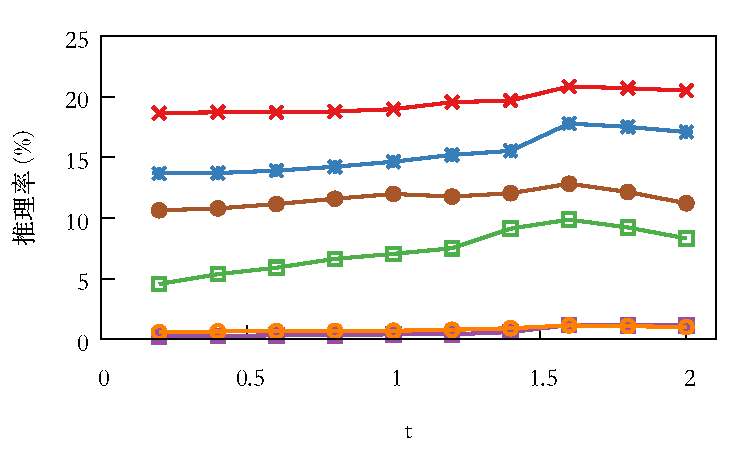
\includegraphics[width=\linewidth]{dis-impact-t-rate.pdf} &
        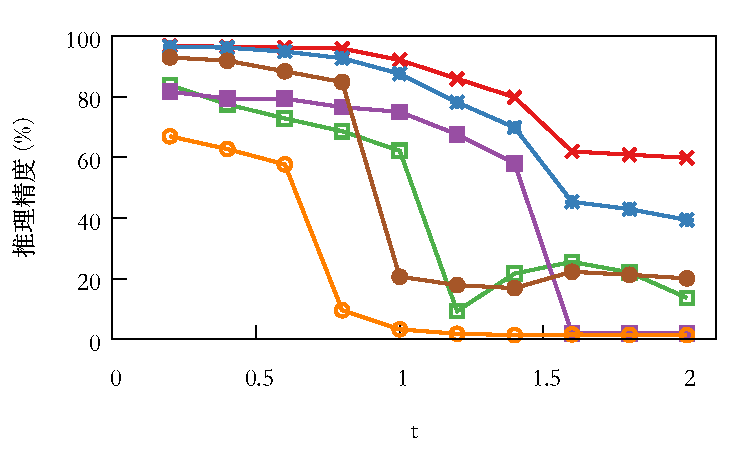
\includegraphics[width=\linewidth]{dis-impact-t-accuracy.pdf}\\
    \end{tabular}
    \caption{基于分布的攻击实验1-参数$t$的变化对推理结果的影响(User004、User013和User015中$u = 128$,User007、User012和User028中$u = 256$;$r = 10$)}
    \label{fig:distribution-impact-t}
\end{figure}

Then, we fix $r$ = 10 and evaluate the impact of $t$.  Figure~\ref{fig:distribution-impact}(c) shows the results. When $t$ is small (e.g., less than 0.5), we observe that the attack misjudges and filters a significant number of ciphertext-plaintext pairs, even they are correct. This introduces {\em false negatives} that reduce the inference rate. As $t$ increases, the number of false negatives decreases.  When $t$ = 1.5, the inference rates hit the maximum values at 21.2\%, 18.2\%, 10.4\%, 1.2\%, 1.2\%, and 13.5\% for User004, User007, User012, User013, User015, and User028, respectively. When $t$ further increases to 2, the corresponding inference rates drop to 20.5\%, 17.1\%, 8.3\%, 1.2\%, 1.0\%, and 11.2\%, respectively. The reason is that if $t$ is too large, it cannot filter false positives effectively. For the same reason, the inference precisions for all users decrease with $t$.  

{\bf Observation (3) --} {\em A smaller $t$ filters a large fraction of false
positives, yet it introduces more false negatives.}   


\subsection{Experiment 2 (Comparison with prior attack):}
We compare the severity of the distribution-based attack with that of the locality-based attack \cite{li17}. In addition to using the FSL dataset like Experiment~1, we include the MS dataset for cross-dataset validation. Specifically, for each MS category, we choose two snapshots at a time, use one to infer the other, and evaluate the average inference rate and precision. 

We consider the following attack instances for comparison. 

\begin{itemize}[leftmargin=*]
\item 
$\tt Baseline$: We re-implement the locality-based attack based on the parameter configuration suggested in \cite{li17}. Specifically, it infers 5 most frequent ciphertext-plaintext pairs in the first invocation (i.e., to initialize a set of ciphertext-plaintext pairs for iteration) of frequency analysis, and 30 in each following invocation (i.e., to iteratively infer ciphertext-plaintext pairs from neighbors).  
\item 
$\tt Distribution$ and $\tt Distribution^S$: We consider two attack instances of the distribution-based attack, denoted by $\tt Distribution^S$ and ${\tt Distribution}$, which operate with and without size information, respectively (i.e., the superscript $\tt S$ indicates that the attack instance operates with size information). We configure $\tt Distribution^S$ and ${\tt Distribution}$ under the same configuration of  ${\tt Baseline}$. In addition, we choose $r$ and $t$ in both  $\tt Distribution^S$ and ${\tt Distribution}$ in the following way: for the FSL dataset, we fix $r$ = 10 for all users, and individually set $t$ = 1.5, 1.2, 1, 1, 0.7, and 0.9 for User004, User007, User012, User013, User015, and User028, respectively; for the MS dataset, we also fix $r$ = 10 for all categories, and set $t$ = 2 for Win7 and Serv-08, and $t$ = 1.6 for Vista-U, Serv-03, and Vista-B, respectively. This is informed by our tests for optimal configurations of the datasets.   
\item 
$\tt Distribution$-$\tt o$ and $\tt Distribution^S$-$\tt o$: We consider two additional distribution-based attack instances, denoted by $\tt Distribution$-$\tt o$ and $\tt Distribution^S$-$\tt o$, which apply the same configurations for $r$ and $t$ as with $\tt Distribution$ and $\tt Distribution^S$, and further use larger $u$ to increase the coverage of inferred ciphertext-plaintext pairs.  Specifically, we configure $u$ in $\tt Distribution$-$\tt o$ and $\tt Distribution^S$-$\tt o$ in the following way:  for the FSL dataset, we apply the same configuration of $u$ in Experiment~1; for the MS dataset, we set $u$ = 128 for Win7, and $u$ = 30 for Serv-03, Serv-08, Vista-B, and Vista-U. 

\end{itemize}

\begin{figure*}[t]
    \centering
    \begin{tabular}{c}
        
\includegraphics[width=.7\textwidth]{pic/legend-fsl-bar.pdf}\\
        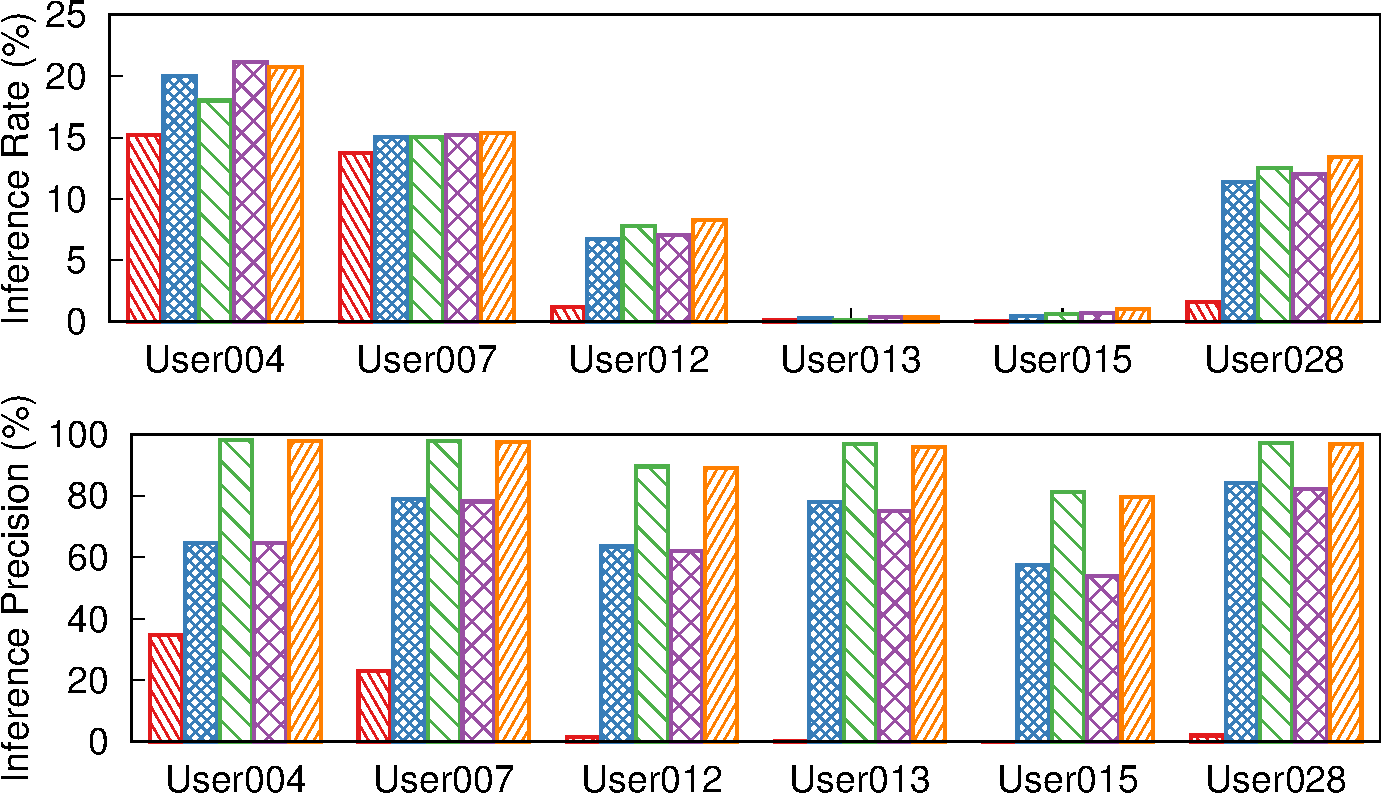
\includegraphics[width=.7\textwidth]{pic/distribution-comparison-fsl.pdf} 
    \end{tabular}
    \caption{Experiment 2 FSL dataset  (Comparison with prior attack): comparison of attack severity for distribution-based attack and locality-based attack.}
    \label{fig:distribution-comparison}
\end{figure*}

\begin{figure*}[t]
    \centering
    \begin{tabular}{c}
        
\includegraphics[width=.7\textwidth]{pic/legend-fsl-bar.pdf}\\
        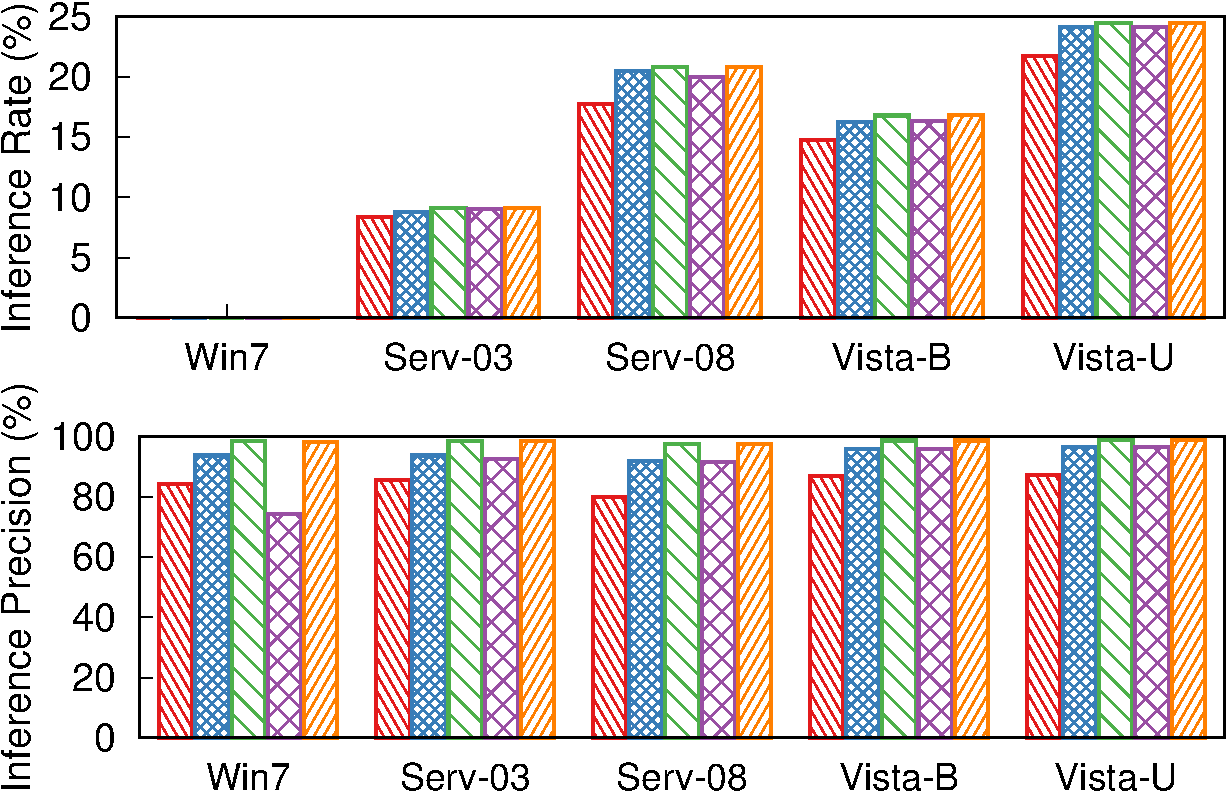
\includegraphics[width=.7\textwidth]{pic/distribution-comparison-ms.pdf}\\
    \end{tabular}
    \caption{Experiment 2 MS dataset (Comparison with prior attack): comparison of attack severity for distribution-based attack and locality-based attack.}
    \label{fig:distribution-comparison}
\end{figure*}


Figure~\ref{fig:distribution-comparison}(a) shows the
comparison results of the FSL dataset. We observe that different instances of
the distribution-based attack outperform the locality-based attack in almost
all cases. For example, regarding User028, the lowest inference rate of the
distribution-based attack is 11.4\%, with the precision of 84.1\% (due to $\tt
Distribution$), while the corresponding inference rate and precision of
$\tt Baseline$ are only 1.2\% and 1.7\%, respectively; this implies that the distribution-based attack reduces the number of false postives by 82.4\% in this case.   

{\bf Observation (4) --} {\em The distribution-based attack significantly
increases the inference precision, while achieving a higher inference rate than
the locality-based attack.} 

$\tt Distribution^S$ and $\tt Distribution^S$-$\tt o$ have higher inference
precisions than $\tt Distribution$ and $\tt Distribution$-$\tt o$,
respectively, since they further filter false positives by size information.
For example, for User004, $\tt Distribution^S$ and $\tt Distribution^S$-$\tt o$  reduce the fraction of false positives in  $\tt Distribution$ and $\tt Distribution$-$\tt o$ from 35.2\% to 1.7\% and from 35.3\% to 2.2\%, respectively. However, in the same case,    
 we observe that the inference rates of $\tt Distribution$ and $\tt Distribution$-$\tt o$ are 20.0\% and 21.2\%, slightly higher than those of  
$\tt Distribution^S$ and
$\tt Distribution^S$-$\tt o$ by 2.0\% and
0.4\%, respectively. The reason is that $\tt Distribution$ and $\tt
Distribution$-$\tt o$ infer a small number of correct results from the
neighbors of incorrect ciphertext-plaintext pairs. In other words,  although
$(C, M)$ is an incorrect ciphertext-plaintext pair, the neighbors of $C$ may
correspond to those of $M$ with a small probability. Even in this case, all distribution-based attack instances are more severe than the locality-based attack instance. Specifically, the inference rate of $\tt Baseline$ is only 15.2\%, lower than those of the best and the worst distribution-based attack instances by 6.0\% and 2.8\%, respectively. 

% For the same reason, $\tt Baseline$ has higher inference rate than $\tt Distribution^S$ in User013.   

{\bf Observation (5) --} {\em Filtering incorrect inference results improves
the inference precision, yet it degrades the coverage of inferred
ciphertext-plaintext pairs and possibly decreases the inference rate.
} 

We further observe that although $\tt Distribution$-$\tt o$ and $\tt
Distribution^S$-$\tt o$ build on larger $u$, their inference rates are just
slightly higher than those of $\tt Distribution$ and $\tt Distribution^S$ by
0.4\% and 0.9\%, respectively. The reason is that the distribution-based
attack iterates inference just through neighbors, and has a bounded coverage
of inferred ciphertext-plaintext pairs. The further increase of $u$ only adds
a small number of new correct  ciphertext-plaintext pairs into results. 

Figure~\ref{fig:distribution-comparison}(b) shows the
results of the MS dataset. Both locality-based and distribution-based attacks
have high inference rates and precisions in most MS categories (except Win7).
The possible reason is that MS snapshots are highly correlated (e.g., the
variance of the total number of chunks is small, as shown in
Table~\ref{tab:dataset}).  We observe that the distribution-based attack still
outperforms the locality-based attack. For example, in Vista-U, the inference
rates and precisions of all inferences of the distribution-based attack are
above 24.1\% and 96.4\%, while those of $\tt Baseline$ are 21.7\% and 87.1\%,
respectively. 

Note that both  distribution-based and  locality-based attacks have low
inference rates (e.g., less than 0.01\%) in the Win7 category. The reason is
 that Win7 includes a large fraction (e.g., more than 98.8\%, as shown in
Table~\ref{tab:dataset}) of unique chunks, which cannot be correctly
inferred by the frequency analysis attacks. 

% We do not include Win7  in the comparison, since all attack instances have low effectiveness. We observe all attacks have higher severity than those in the FSL dataset.   



\begin{figure*}[t]
     \centering
    \centering
    \begin{tabular}{c}
        
\includegraphics[width=.35\textwidth]{pic/legend-effectiveness.pdf}\\
        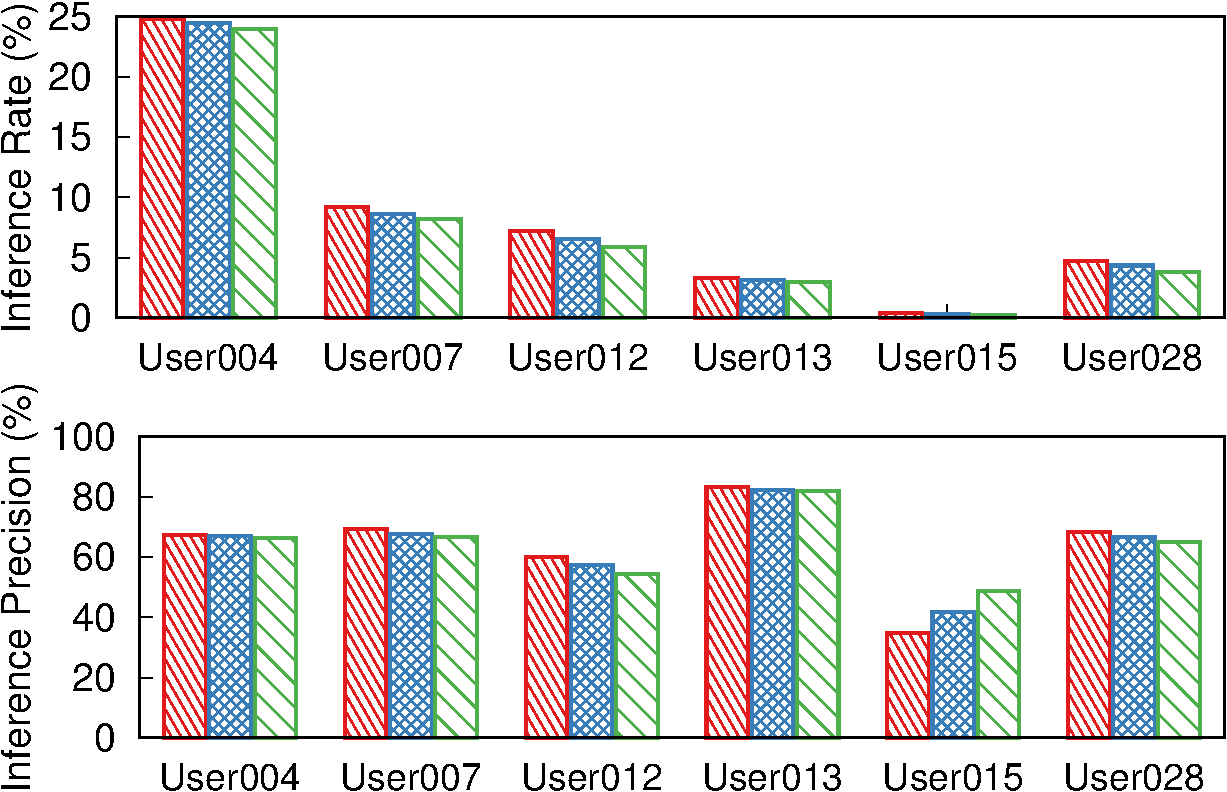
\includegraphics[width=.7\textwidth]{pic/distribution-effectiveness-wo-size.pdf}
    \end{tabular}
	\caption{Experiment 3 Distribution-based attack without size information  (Attack effectiveness): severity of distribution-based attack in FSL dataset.}
	\label{fig:experiment-distribution-effectiveness}
\end{figure*}

\begin{figure*}[t]
     \centering
    \centering
    \begin{tabular}{c}
        
\includegraphics[width=.35\textwidth]{pic/legend-effectiveness.pdf}\\
        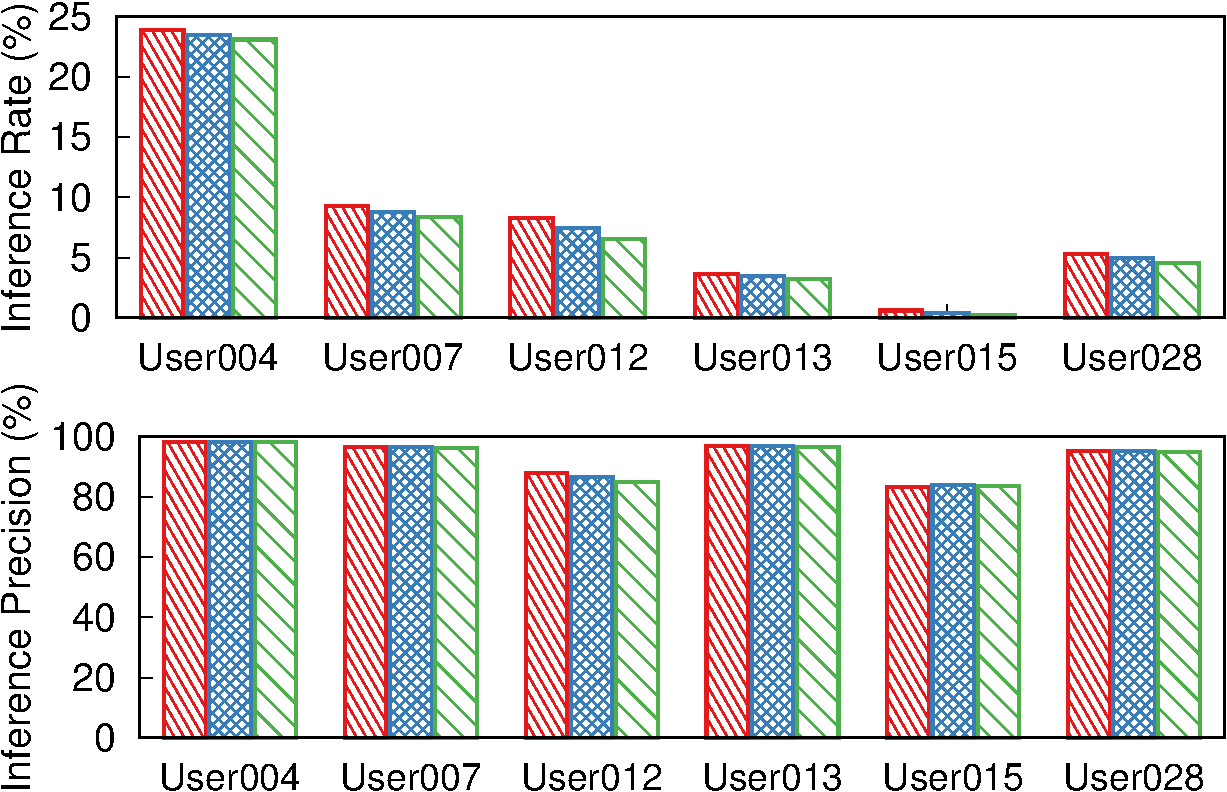
\includegraphics[width=.7\textwidth]{pic/distribution-effectiveness-w-size.pdf}
    \end{tabular}
	\caption{Experiment 3 Distribution-based attack with size information (Attack effectiveness): severity of distribution-based attack in FSL dataset.}
	\label{fig:experiment-distribution-effectiveness}
\end{figure*}



\subsection{Experiment 3 (Attack effectiveness):} We consider a long-term
backup scenario and examine the effectiveness of the distribution-based attack
with the FSL dataset. Specifically, we choose the $i$th FSL weekly backup of
each user as the auxiliary information to infer original plaintexts in the corresponding $(i+w)$th FSL
weekly backup. Clearly, the smaller $w$ is, the higher correlation between the
auxiliary information and the target backup will be.  We configure the two  
distribution-based attack instances $\tt Distribution$-$\tt o$ and $\tt Distribution^S$-$\tt o$
like Experiment~2, and evaluate their inference rates and inference precisions that
are averaged for all available $i$ for each user. 

Figure~\ref{fig:experiment-distribution-effectiveness}(a) shows the results. The
distribution-based attack has varying inference rate and precision  across
users. For example, in the favorable case like User004, it achieves the
highest inference rates of 24.8\%, 24.5\%, and 24.0\% with the precisions of
67.3\%, 67.0\%, and 66.5\% for $w$ = 1, 2, and 3, respectively; in the
non-favorable case like User015, the inference rate of the distribution-based
attack is only around 0.3\%. The possible reason is that the backup data from
User015 has low chunk locality. 

In addition, we observe that the correlation (i.e., $w$) of the auxiliary
information has low impact on the effectiveness of the distribution-based
attack.  For example, when $w$ increases from 1 to 3, it only leads to limited
degradations on inference rate (e.g., less than 1.4\%) and precision (e.g.,
less than 5.6\%). The reason is that the distribution-based attack addresses
disturbances to frequency ranking and preserves attack effectiveness.  

{\bf Observation (6) --} {\em The distribution-based attack can limit the
degradation of attack effectiveness in the presence of loosely correlated
auxiliary information.} 

% We also use the instance in Experiment 2 to evaluate the effectiveness of the distribution-based attack that operates with
 % size information. 
 Figure~\ref{fig:experiment-distribution-effectiveness}(b) shows the results of $\tt Distribution^S$-$\tt o$. We observe that it has similar inference rate with $\tt Distribution$-$\tt o$,  
 while achieving much higher precision. For example, the average inference precision of all users are 93.1\%, 92.8\%, and 92.4\% for $w$ = 1, 2, and 3, respectively.  

% Figure~\ref{fig:experiment-distribution-severity-ms} shows the attack results of the MS dataset. The distribution-based attack achieves high severity. For example, it can infer 24.0\% of unique chunks in Vista-U with a precision of 96.2\%.    

% Although there is l          

\section{Results of Clustering-based Attack}
\label{sec:experiment-clustering}




\subsection{Experiment 4 (Impact of parameter):} We first evaluate the impact
of the parameter $k$, which defines the upper bound distance
in combining the closest clusters.  We use both the FSL and the VM datasets to
study how $k$ affects the underlying clustering scheme in the attack.
Specifically, we apply segmentation on the last backup of each considered FSL
and VM user, respectively, and generate the segments that have a fixed size of
4MB. 

The clustering scheme aims to aggregate similar ciphertext segments into the
same cluster, without compromising the confidentiality of chunks in each
ciphertext segment.  To quantify its effect, we compare the results of
clustering with those of a {\em real} classification approach, which directly
classifies segments by their minimum chunk hash.  Suppose we generate $m$ real
classes of segments by classification, and $\widetilde{m}$ clusters by the
clustering scheme, respectively.  We consider {\em clustering closeness},
evaluated by $\frac{{\sf abs}(m-\widetilde{m})}{m}$ (where 
${\sf abs}(m-\widetilde{m})$ returns the absolute value of $m-\widetilde{m}$),
which quantifies how the  number of clusters approximates that of real
classes. In addition, let $\hat{m}$ be the number of clusters, in which all
segments are similar (i.e., have the same minimum chunk hash). We also
consider {\em clustering correctness}, evaluated by
$\frac{\hat{m}}{\widetilde{m}}$, which quantifies how precisely the clustering
scheme groups similar segments.  

Figure~7(a) shows the results of the FSL dataset, where we
consider four FSL users (e.g., User004, User007, User015 and User028) for
saving evaluation time. The clustering closeness first increases with $k$,
since the number (i.e., $\widetilde{m}$) of clusters decreases and
approximates $m$. When $k$ increases further, the number of clusters drops
away from $m$, and leads to the increase of clustering closeness.  In
addition, we observe that the clustering correctness gradually decreases with
$k$, because some of non-similar segments (i.e., their minimum chunk hashes are
different) are aggregated into the same cluster. Both results suggest that we
can configure an appropriate $k$ to balance the closeness and correctness of
clustering. For example, when we set $k$ = 0.65 for User015, the corresponding
closeness and correctness are 1.0\% and 94.2\%, respectively. This implies
that the results of the clustering scheme  highly approximates
those of real classification.             

{\bf Observation (7) --} {\em By configuring an appropriate $k$ for
clustering, we  approximate the results of  classifying segments, without the knowledge of  minimum chunk hash in each
segment.}   

Figure~7(b) shows the results of the VM dataset. We observe
that the clustering closeness and correctness of all VM users have  similar
tendencies with those of FSL users. When we configure $k$ = 0.8, the average
clustering closeness of all VM users is only 3.0\%, while the corresponding
clustering correctness is as high as 93.1\%.     


\begin{figure*}[t]
\centering
    \begin{tabular}{cc@{\hspace{0.3in}}p{.32\textwidth}}
    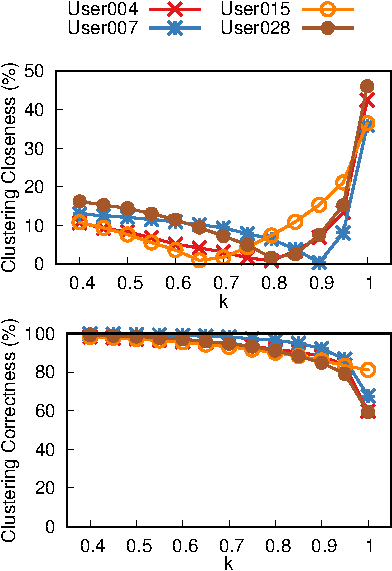
\includegraphics[width=.3\textwidth]{pic/clustering-impact-d-fsl.pdf} &
    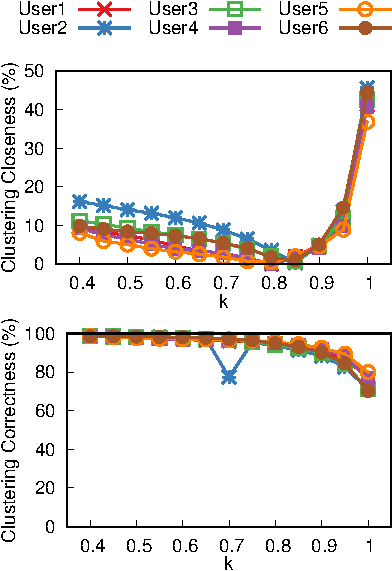
\includegraphics[width=.3\textwidth]{pic/clustering-impact-d-vm.pdf} & 
    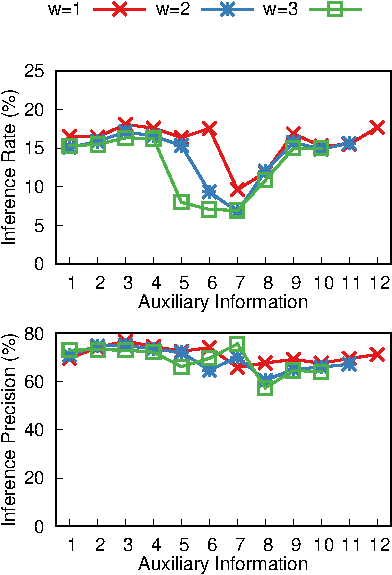
\includegraphics[width=.3\textwidth]{pic/clustering-effectiveness.pdf} \medskip \\
{\footnotesize 
        (a) FSL dataset } 
&
{\footnotesize 
        (a) VM dataset } 
        &  ~~~ \medskip \\
        \multicolumn{2}{p{.64\textwidth}}{
            \footnotesize Fig.~7\quad Experiment 4 (Impact of parameter): impact of $k$ in the clustering scheme; for clustering closeness, the smaller the better; for clustering correctness, the larger the better. } &
        % \multicolumn{2}{c}{\footnotesize Fig.~6\quad Experiment 4 (Impact of parameter): show impact of $d$ with clustering closeness and correctness; for clustering closeness, the smaller the better; for clustering correctness, the larger the better.} &
        {\footnotesize
Fig.~8\quad Experiment 5 (Attack effectiveness):  severity of clustering-based attack in VM dataset.
        }
\end{tabular}
    \hspace{-1in}
\end{figure*}

% \begin{figure}
% 	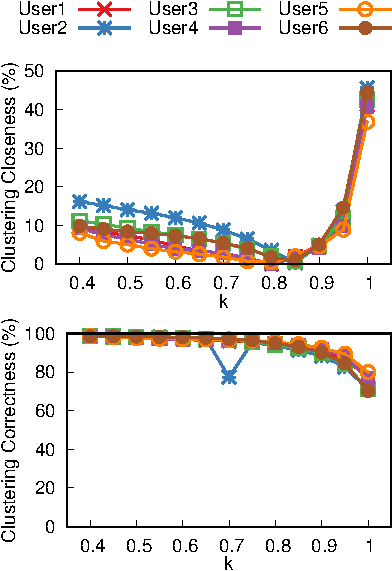
\includegraphics[width=.48\textwidth]{pic/clustering-impact-d.pdf}
% 	\caption{Experiment 6 (Impact of parameter).}
% 	\label{fig:experiment-clustering-impact}
% \end{figure}

\begin{table*}[!t]
\small
    \caption{Experiment 6 (Security implications)}
\renewcommand{\arraystretch}{1.2}
\vspace{-3pt}
 \begin{minipage}[t]{0.7\textwidth}
\centering
        (a) Distribution-based attacks \medskip \\
\begin{tabular}{|c|c|c|c|c|c|}
\hline

    \multirow{2}{*}{\bf Type} & \multirow{2}{*}{\bf Extension Name} & \multirow{2}{*}{\bf \centering Range of File Size}  & \multicolumn{2}{c|}{\bf Raw Inference Rate} \\ \cline{4-5} 
    & & &  $\sf Distribution$-$\sf o$ & $\sf Distribution^S$-$\sf o$ \\ \hline
\hline
    Office & doc(x), ppt(x), xls(x) & 10KB-1MB   & 4.9\% & 5.3\%\\
\hline
    Picture & jpg, png &10-100KB  & 7.7\% & 6.7\% \\
\hline
    Source & c, h, cpp, java, py & 10-20KB   & 17.1\% & 15.0\%\\
% \hline
	% Library & .a, .dll, .so \\
% \hline
	% Compression & .bz2, .gz, tar, rar, zip, 7z \\
\hline
    Database & db, po & 20-700KB   & 2.6\% & 2.4\%\\
\hline
    Disk & vmdk, img & 200MB-1GB  & 15.8\% & 16.7\%\\
\hline
\end{tabular}
\label{tab:file}
 \end{minipage}
\hfill
    \begin{minipage}[t]{0.3\textwidth}
    \centering
        (b) Clustering-based attack \medskip \\
    \begin{tabular}{|c|c|}
    \hline
        {\bf Users} & {\bf Raw Inference Rate} \\
    \hline
    \hline
        1 & 13.2\% \\ 
    \hline
        2 & 22.4\% \\ 
    \hline
        3 & 25.7\% \\ 
    \hline
        4 & 28.4\% \\ 
    \hline
        5 & 18.5\% \\ 
    \hline
        6 & 30.8\% \\ 
    \hline
    \end{tabular}
\label{tab:user}
    \end{minipage}

\end{table*}



\subsection{Experiment 5 (Attack effectiveness):} We now study the
effectiveness of the clustering-based attack. Due to the boundary shift of
fixed-size segment, it has low effectiveness
(about 1\% inference rate in our test) against the FSL dataset.  Thus, we use
the VM dataset to examine its severity. To configure the attack, we set $k$ =
0.8 for clustering, and $(u, r, t)$ = (5000, 100, 0.5) for relating ciphertext
clusters to corresponding plaintext clusters.  

In our micro-benchmarking, we find that the chunk-level inference in the
clustering-based attack only infers thousands of chunks correctly, which
contributes to a negligible inference rate (e.g., less than 0.01\%).  
% The
% reason is that each cluster includes a large number of chunks, and frequency
% analysis is ineffective in this case. 
Thus, we focus on the
segment-level inference, which presents the bottom line of severity in the
clustering-based attack. To be consistent with the chunk-level measurements, we count inference rate and precision based
on the unique chunks in each correctly inferred segment. 

We use the same evaluation methodology of Experiment~3, and report the results
in Figure~8. Specifically, the x-axis describes the index $i$ (where 1 $\leq i \leq$
12) of the VM backup that is used as the auxiliary information for attack,
while the y-axis presents the average inference rate or precision of all VM
users against the $(i+w)$th backup (where $w$ = 1, 2, and 3). We observe that both the inference rate and the inference
precision fluctuate significantly. For example, when using the 3rd backup as
the auxiliary information, the attack achieves the highest inference rates at
18.1\%, 17.1\% and 16.3\%, with the precisions of 76.8\%, 75.0\% and 73.0\%
for $w$ = 1, 2, and 3, respectively. 
On the other hand, when using the 7th
backup as the auxiliary information, the corresponding inference rates and
precisions drop down to 9.6\% and 65.9\%, 6.8\% and 71.2\%, and 6.9\% and
75.6\%, respectively. The reason is that the VM users have heavy updates after
the 7th week, and this reduces the correlation  of adjacent backups. 
On
average, for $w$ = 1, 2 and 3, the clustering-based attack infers 15.8\%,
14.0\%, and 12.6\% ciphertext-plaintext pairs, with the precisions of 71.1\%,
69.1\%, and 68.9\%, respectively. 
% This demonstrates high severity against
% the VM disk images.   

\section{Results of Security Implications}
\label{sec:case}
We thus far have examined the severity of inference attacks by quantifying the
correctly inferred ciphertext-plaintext pairs.  However, it remains an open
issue that what are the security implications informed by these results and
how the frequency analysis attacks bring actual damage. In the following
experiment, we evaluate the security implications of our attacks based on the
{\em raw inference rate}, defined as the percentage of raw data content
affected by correctly inferred chunks.   




\subsection{Experiment 6 (Security implications):}
We first consider the distribution-based attack, and evaluate its raw
inference rate against {\em different types} of files. We drive the evaluation
using the FSL dataset, since only the FSL dataset includes file metadata (that
includes the extension names of files) in plaintext. Specifically, we focus on
five types of files that have specific extension names (see
Table~\ref{tab:file}(a)): office files ({\em Office}), picture files 
({\em Picture}), programming source files ({\em Source}), database files 
({\em Database}), and disk image files ({\em Disk}). These files occupy more
than 60\% of raw content of FSL snapshots.   

We apply the methodology of Experiment~2, and evaluate the raw inference
rates of $\sf Distribution^S$-$\sf o$ and $\sf Distribution$-$\sf o$. 
Table~\ref{tab:file}(a) shows the results. Both attack instances have high raw
inference rates against {\em Disk} (e.g., 15.8\% for 
$\sf Distribution$-$\sf o$ and 16.7\% for $\sf Distribution^S$-$\sf o$),
because each disk file includes a large number of rarely updated chunks that
form high locality within the same file. Interestingly, we observe that 
{\em Source}, although each file is of a small size, also incurs high raw
inference rates by the distribution-based attacks (e.g., 17.1\% for 
$\sf Distribution$-$\sf o$ and 15.0\% for $\sf Distribution^S$-$\sf o$). The
reason is that programming source files are often stored together in file system
(e.g., the source files that belong to the same project locate in an identical
directory) and form a large stretch of correlated chunks, which present high
locality across files. For small and scattered files (e.g., {\em Office}, 
{\em Picture}, and {\em Database}), the distribution-based attacks have
relative low raw inference rates.     


{\bf Observation (8) --} {\em The severity of the distribution-based attack depends on the update frequencies, sizes, and spatiality of target files. } 

We examine the security implication of the clustering-based attack using the VM dataset. Specifically, we use the 11th  backup of each VM user  to infer original content in corresponding 13th VM backup. Since the VM dataset does not contain any metadata, we count the raw inference rate based on the  whole data content in each VM snapshot. Note that we filter all zero chunks in the count of raw inference rate, because they occupy a large fraction in VM disk images \cite{jin09}.           


% switch to the clustering-based attack, and infer the content of the last (i.e., the 13th) VM backup based on the corresponding 11th backup. Since the VM dataset does not contain metadata, we evaluate the raw inference rate across different users. Specifically, like Experiment 7, we only consider segment-level attack for high precision, and count the raw inference rate based on the correctly inferred segments. Note that since VM images commonly contain a large fraction of zero chunks ,  we filter out the zero segments in our inferred raw content.    

We use the same configuration of Experiment~5, and evaluate raw inference rate
based on segment-level inference.  Table~\ref{tab:user}(b) shows the results
for different users.  We observe that the clustering-based attack achieves high
severity against the VM dataset. For example, it infers up to 30.8\% raw
content of User6's VM backup. On average, the raw inference rate of all users
is as high as 23.2\%.  
% a relatively high raw inference rate.  On average, the raw inference rate is 23.2\% for all users. 

{\bf Observation (9) --} {\em The clustering-based attack threatens the
confidentiality of VM disk images. } 

